\section{Ada Code to Configure the GPIO}

We now need to configure the \gls{ps} GPIO \gls{emio} pins as outputs by writing the GPIO controller’s direction and output-enable registers, then write the data registers to drive the bits high or low. From the \href{https://docs.amd.com/r/en-US/ug585-zynq-7000-SoC-TRM/Introduction?tocId=qKswejA9UtbWtFx59v3r_g}{Zynq 7000 SoC Technical Reference Manual (UG585)}, the introduction to section General Purpose I/O reads: 

\begin{quotation}
    The general purpose I/O (GPIO) peripheral provides software with observation and control of up to 54 device pins via the MIO module. It also provides access to 64 inputs from the Programmable Logic (PL) and 128 outputs to the PL through the EMIO interface. The GPIO is organized into four banks of registers that group related interface signals.

    Each GPIO is independently and dynamically programmed as input, output, or interrupt sensing. Software can read all GPIO values within a bank using a single load instruction, or write data to one or more GPIOs (within a range of GPIOs) using a single store instruction. The GPIO control and status registers are memory mapped at base address 0xE000\_A000.
\end{quotation}

The last senetence is of particular importance as it tells us the base address of the GPIO control and status regsiters we must work from. Further, the \gls{emio} GPIOs are connected to banks 2 and 3

\begin{center}
   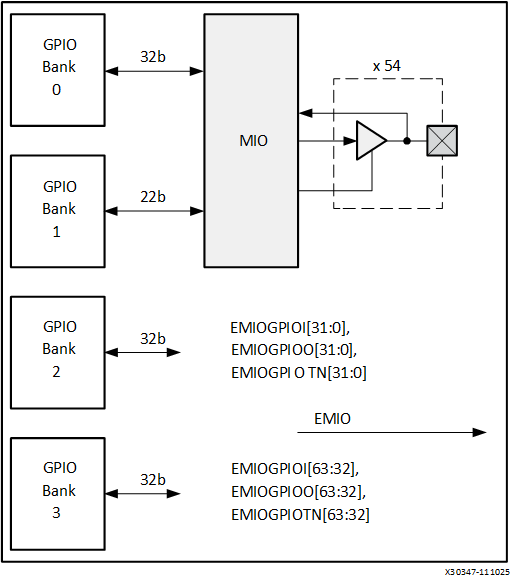
\includegraphics[width=0.9\textwidth]{../Figures/Blink_LED/write_to_gpio/EMIO_banks.png}
\end{center}

From our board diagram, we know that we are using \gls{emio} GPIO\_O(7:0) output port i.e. bits 7 downto 0 of the \gls{emio}, which we have connected to the rtl with via the port o\_leds (Fig. \ref{fig: w_2_gpio BD}).

\begin{figure}
    \centering
    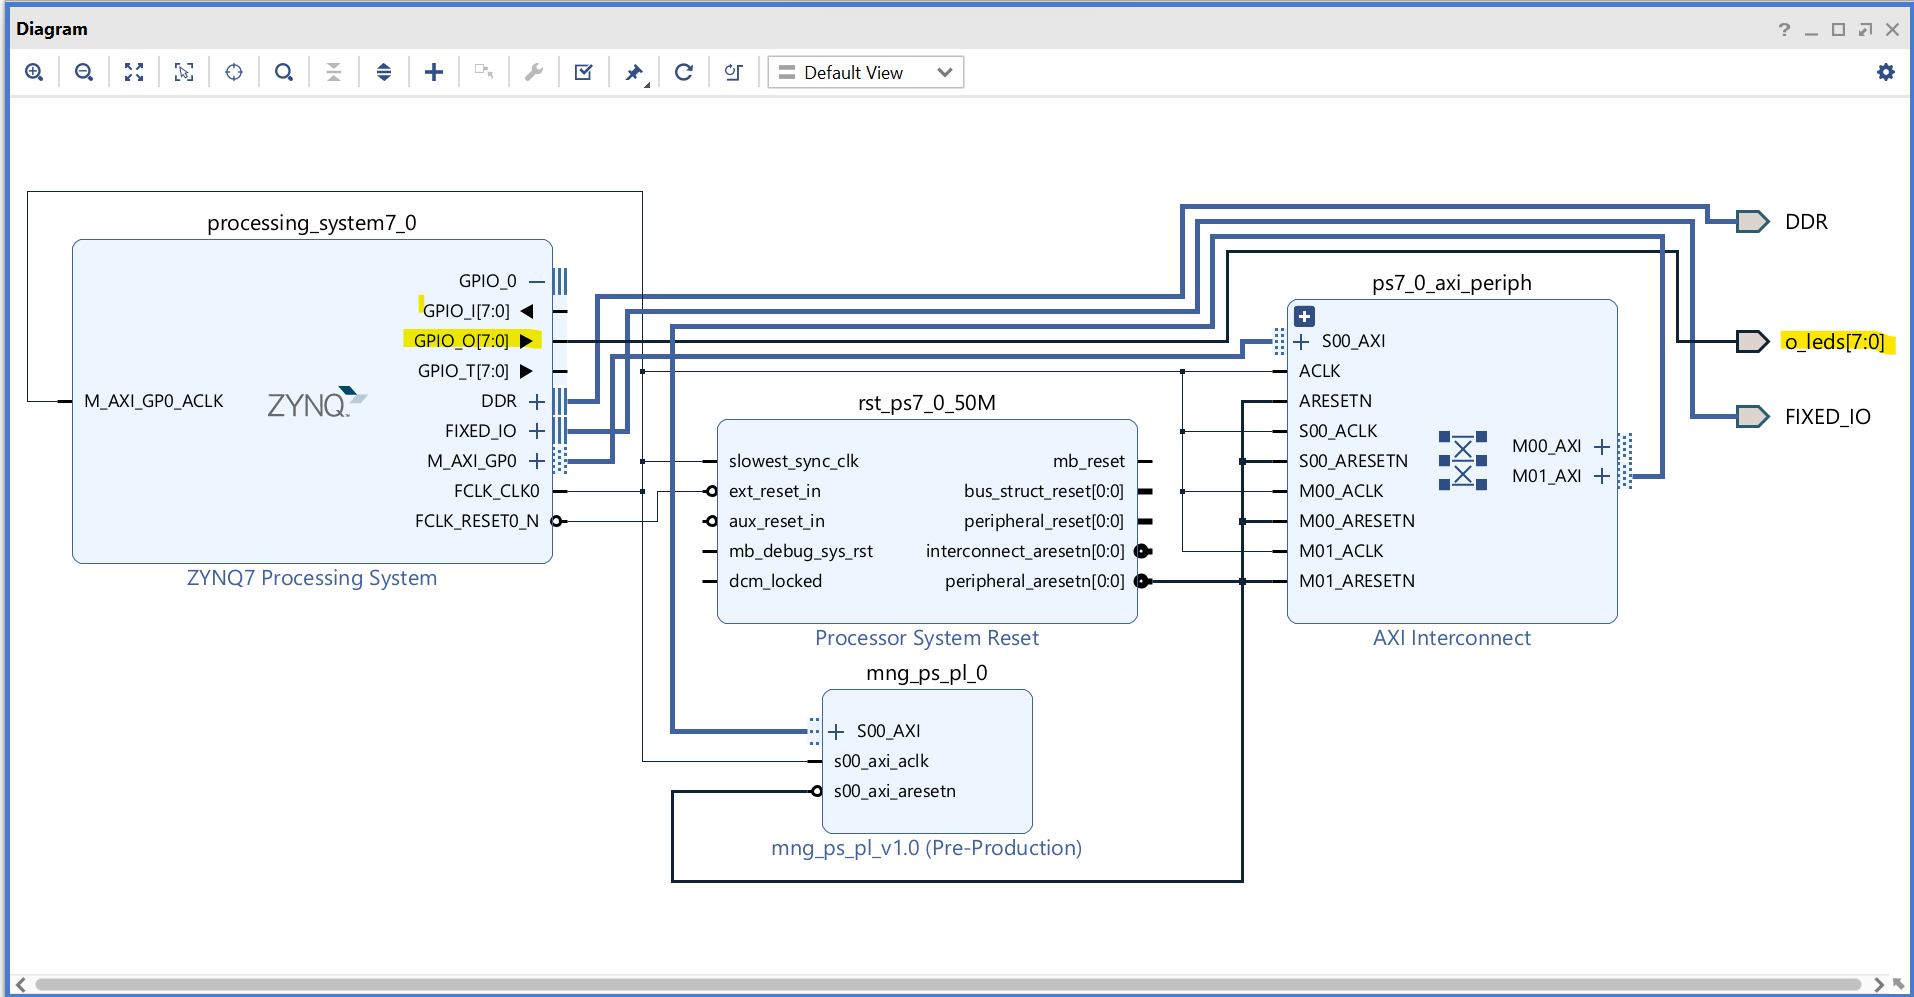
\includegraphics[width=0.9\textwidth]{../Figures/Blink_LED/write_to_gpio/gpio_0_o_leds.png}
    \caption{We have connected the \gls{emio} GPIO\_O register to o\_leds. Here, GPIO\_I: Input to PS ← comes from PL, GPIO\_O: Output from PS → goes into PL, GPIO\_T: Tri-state control (direction control). We only need GPIO\_O.  }\label{fig: w_2_gpio BD}
\end{figure}

 To send data to our LED, then, we must find in the register map (under section \href{https://docs.amd.com/r/en-US/ug585-zynq-7000-SoC-TRM/Register-Summary?tocId=vG2VoctF9y37ZhrdSUcBAw}{Register Summary of UG585}) the correct control registers to control GPIO\_O. 


Since EMIO[0:31] is bank 2, we find the correct registers are (Fig. \ref{fig: w_2_gpio reg_map})  

\begin{table}[h!]
\centering
\begin{tabular}{|l|c|c|c|c|l|}
\hline
\textbf{Name} & \textbf{Offset} & \textbf{Width} & \textbf{Access} & \textbf{Reset} & \textbf{Description} \\ \hline
DATA\_2 & 0x00000048 & 32 & rw & 0x00000000 & Output Data (GPIO Bank2, EMIO) \\ \hline
DIRM\_2 & 0x00000284 & 32 & rw & 0x00000000 & Direction mode (GPIO Bank2, EMIO) \\ \hline
OEN\_2  & 0x00000288 & 32 & rw & 0x00000000 & Output enable (GPIO Bank2, EMIO) \\ \hline
\end{tabular}
\caption{GPIO Bank2 (EMIO) Register Map}
\label{tab:gpio_bank2}
\end{table}

\begin{figure}
    \centering
    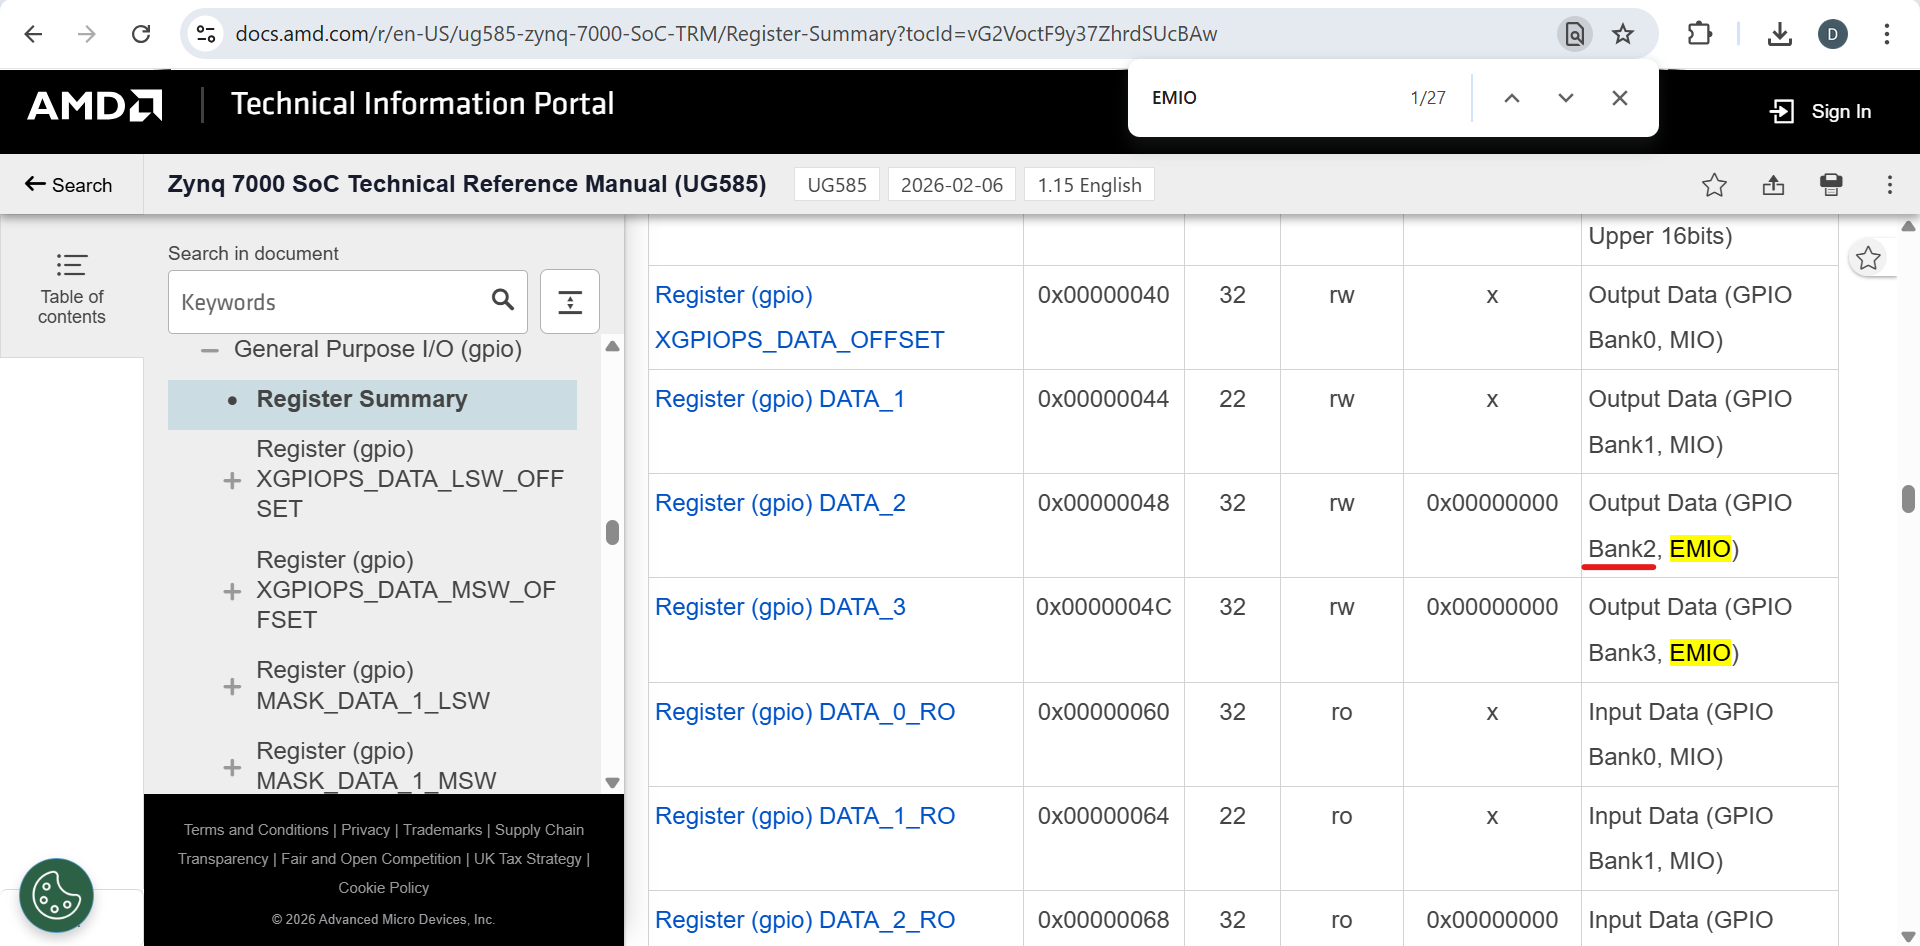
\includegraphics[width=0.9\textwidth]{../Figures/Blink_LED/write_to_gpio/data_reg.png}
    \caption{We need to find the EMIO GPIO register to output data. We find it is at offset 0x48, it is 32 bits, it is read/write (rw) and it resets to 0x0.}\label{fig: w_2_gpio reg_map}
\end{figure}

Thus, in software we must:

\begin{enumerate}
    \item Set direction output => Set bit 0 in DIRM\_2
    \item Enable output => Set bit 0 in OEN\_2
    \item Write value => Set/clear bit 0 in DATA\_2
\end{enumerate}